\subsection{Stream Testing}
To address \textbf{RQ1} and \textbf{RQ3} two groups were assigned the task to model a Controller for PacMan and SuperMario respectively and interview the results afterwards. In the future the groups will be referred to as \textit{group A} and \textit{group B}. Group A consists of one subject who is familiar with EmbeddedMontiArc and group B consists of two subjects who have no experience with EmbeddedMontiArc. These groups were selected random among the students of a computer science seminar. 

EmbeddedMontiArc comes along with stream tests in order to check a component against a condition as stated in the previous chapter.
We can use those tests to define the conditions the controllers need to fulfill. Those conditions are taken from use cases scenarios. For PacMan the most general acceptance test would be to never let the PacMan die. Due to the fact that stream tests cannot be defined unlimited and that this test might be hard to fulfill the following deterministic tests for PacMan and SuperMario were defined.

\subsubsection{PacMan}
The tests are taken from use case scenarios as stated before. In this section the process of deriving the stream test from a scenario is presented once and then a few conditions are framed. \newline

\emph{Deriving a Stream Test} \newline
In fig. \ref{fig:pacManFleeing} a scenario is shown where the only option for PacMan is to flee to the left in order to not collide with the pink and blue ghost. The values of the ghosts and PacMan are partially listed in listing \ref{lst:pmStreamValues}. Together with the other values this concludes to the stream test shown below \ref{lst:pmStreamTest}.
\begin{figure}[!h]
	\centering
	\subfigure[]{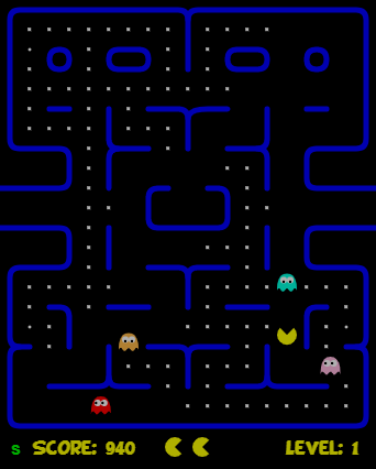
\includegraphics[width=0.49\textwidth]{pictures/PacMan/StreamTests/2/Bild1.PNG}} 
	\subfigure[] {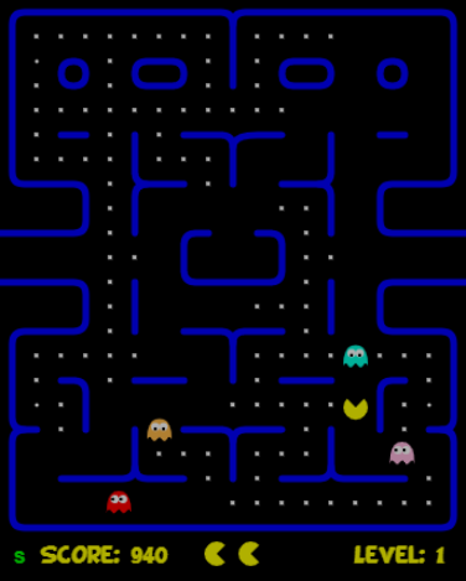
\includegraphics[width=0.49\textwidth]{pictures/PacMan/StreamTests/2/Bild2.PNG}} 
	\subfigure[]{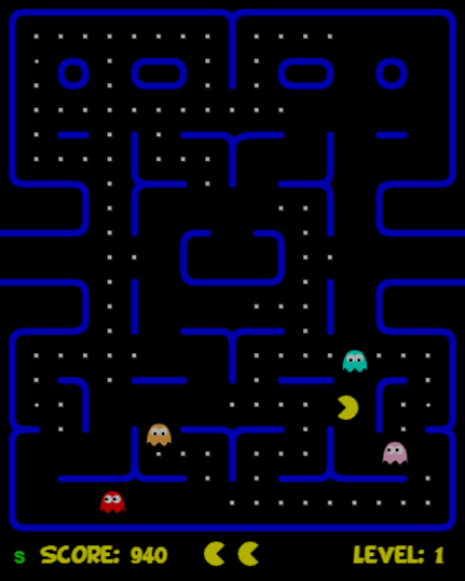
\includegraphics[width=0.49\textwidth]{pictures/PacMan/StreamTests/2/Bild3.PNG}} 
	\subfigure[]{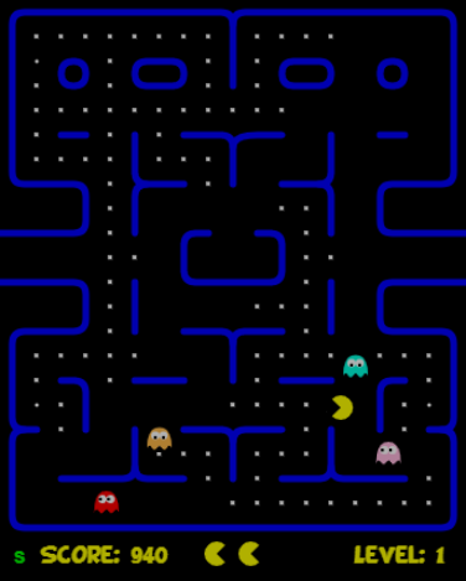
\includegraphics[width=0.49\textwidth]{pictures/PacMan/StreamTests/2/Bild4.PNG}} 
	\caption{PacMan has to move left to avoid colliding with the ghosts} 
	\label{fig:pacManFleeing}
\end{figure}
\begin{lstlisting}[caption={Values for the stream test},label=lst:pmStreamValues, frame=single]
(a)
  PacMan: (15m, 17.2m) 
  Pink Ghost: (17m, 19m) 
  BlueGhost: (15m, 14.8m) 
  newDir: 0
(b)	
  PacMan: (15m, 17m) 
  Pink Ghost: (16.8m, 19m) 
  BlueGhost: (15m, 15m) 
  newDir: 0
(c)	
  PacMan: (14.8m, 17m) 
  Pink Ghost: (16.6m, 19m) 
  BlueGhost: (15m, 15.2m) 
  newDir: 2
(d)	
  PacMan: (14.6m, 17m) 
  Pink Ghost: (16.4m, 19m)
  BlueGhost: (15m, 15.4m)
  newDir: 2
\end{lstlisting}

\begin{lstlisting}[caption={Stream test for the scenario above},label=lst:pmStreamTest, frame=single, morekeywords={tick, stream, for, package}]
package de.rwth.pacman;
stream Test1 for PacManWrapper {
  ghostX: [5.4m,15m,17m,7m] tick [5.2m,15m, ...
  ghostY: [21m,14.8m,19m,17.2m] tick [21m,15m, ...
  ghostDirection: [2,1,2,1] tick [2,1,2,1] tick ...
  ghostEtable: [false, false, false, false] tick ...
  ghostEaten: [false, false, false, false] tick ...
  pacManX: 15m tick 15m tick 14.8m tick 14.6m;
  pacManY: 17.2m tick 17m tick 17m tick 17m;
  pacManEaten: false tick false tick false tick false;
  pacManLives: 3 tick 3 tick 3 tick 3;
  pacManScore: 0 tick 0 tick 0 tick 0;
  map: [0,0,0,0,0,0,0,0,0,0,0,0,0,0,0,0,0,0,0; ...
  newPacManDirection: 0 tick 0 tick 2 tick 2;
}
\end{lstlisting}

\emph{Some other tests}\newline
To formulate just some tests, here are a few examples:
\begin{itemize}
	\item If PacMan is located at an intersection and ghosts are coming from two sides, PacMan should walk to a safe path.
	\item If PacMan is located at an intersection and ghosts are at the top path and are all eatable, PacMan should walk this path.
	\item If PacMan is located at an intersection and there are ghosts from 3 directions and in the other direction there is a ghost facing away from PacMan, PacMan should walk this direction.
	\item If there are no ghosts nearby, PacMan should walk the direction with the largest biscuit/coin value.
\end{itemize}

Those scenarios can be tested easily within a few ticks via stream testing.

\subsubsection{Supermario (by Philipp Haller)}
The goal for the Supermario model is to solve a level successfully. The first level was chosen since it provides a diverse environment with different enemy types and obstacles, while not being too skill intensive to solve. 
Prior to modeling some assumptions were made to fulfill time and complexity constraints.
Only a fixed number of enemies and obstacles in the path of the player are considered in order to ensure a static input size. For this number, five has proved to be sufficient for the first level and the implemented strategy. There are rarely more than 3 enemies in scene. For the same reason only the next hole in the ground is considered.
In order to develop the model, different situations were assessed and according tests derived. Both the scenarios which a Supermario model has to master and the derived tests are listed below.

\begin{figure}[!h]
	\centering
	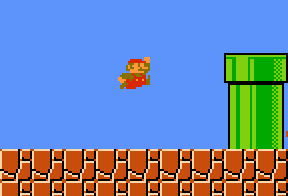
\includegraphics[scale=0.55]{pictures/haller_mario1.PNG}
	\caption{Mario has to jump and move right to overcome the obstacle}
	\label{fig:marioobstacle}
\end{figure}

Figure \ref{fig:marioobstacle} depicts the player next to an obstacle. In order to jump over it he has to move right and jump at the same time. He needs to keep jumping until he is higher than the obstacle.

\begin{figure} 
	\centering
    \subfigure[Mario evades a enemy by jumping]{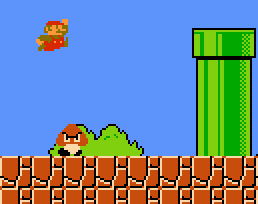
\includegraphics[height=0.3\textwidth]{pictures/haller_mario2.PNG}} 
    \subfigure[Mario defeats enemies by landing on them]{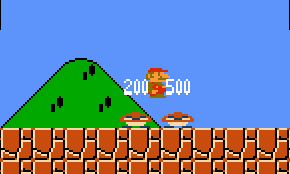
\includegraphics[height=0.3\textwidth]{pictures/haller_mario3.PNG}} 
	\caption{Mario has to jump over/to enemies} 
	\label{fig:marioenemies}
\end{figure} 

Figure \ref{fig:marioenemies} shows two situations. In the first one, mario jumps to evade an enemy. The second depicts him landing on top of enemies to kill them.

\begin{figure} 
	\centering
    \subfigure[Mario and a hole in the ground]{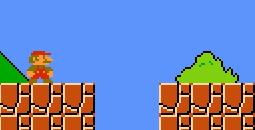
\includegraphics[height=0.3\textwidth]{pictures/haller_mario4.PNG}} 
    \subfigure[Mario and a hole with obstacles]{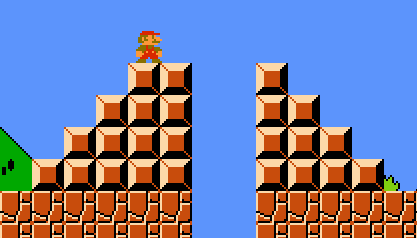
\includegraphics[height=0.3\textwidth]{pictures/haller_mario5.PNG}} 
	\caption{Mario has to jump over a hole} 
	\label{fig:mariohole}
\end{figure} 
In Figure \ref{fig:mariohole} the player is seen standing next to holes in the ground. In the first picture he is on the ground level, in the second he is standing on an obstacle.

The stream tests derived from the scenarios are introduced in the following.
\begin{lstlisting}[label=lst:enemywatchertest_1, caption=Enemy watcher stream test, morekeywords={package, stream, tick, for},
frame=single, basicstyle=\small]
package de.rwth.supermario.haller.environment;

stream Env_EnemyWatcher_Evade for EnemyWatcher {
    EnemyDistX:         200 tick    100     tick     75;
    EnemyDistY:           0 tick      0     tick      0;
    EnemyVelocityX:     -10 tick    -10     tick    -10;
    EnemyVelocityY:       0 tick      0     tick      0;
            
    movesTowardsPlayer:   1 tick      1     tick      1;
    inJumpRange:          0 tick      0     tick      1;
    }
\end{lstlisting}
If a enemy gets closer than 80 pixels (two blocks) and is on the same height as the player, the player has to jump in order to evade the enemy (listing \ref{lst:enemywatchertest_1}). The units for the EnemyDistX and EnemyDistY values are pixels, while the velocities are given in pixels per time frame.
The output values are of type boolean.

\begin{lstlisting}[label=lst:enemywatchertest_2, caption=Enemy watcher stream test, morekeywords={package, stream, tick, for},
frame=single, basicstyle=\small]
package de.rwth.supermario.haller.environment;

stream Env_EnemyWatcher_FromAbove for EnemyWatcher {
        
    EnemyDistX:         200 tick    100     tick      5;
    EnemyDistY:         128 tick    128     tick     32;
    EnemyVelocityX:     -10 tick    -10     tick    -10;
    EnemyVelocityY:       0 tick      0     tick      0;
            
    movesTowardsPlayer:   1 tick      1     tick      1;
    inJumpRange:          0 tick      0     tick      0;

    }
\end{lstlisting}
The stream in listing \ref{lst:enemywatchertest_2} covers the case when the player is above enemies and shall drop on them while he is above.



\begin{lstlisting}[label=lst:enemywatchertest_3, caption=Enemy watcher stream test, morekeywords={package, stream, tick, for},
frame=single, basicstyle=\small]
package de.rwth.supermario.haller.environment;

stream Env_EnemyWatcher_FromAbove for EnemyWatcher {
        
    EnemyDistX:         -1 tick;
    EnemyDistY:         -1 tick;
    EnemyVelocityX:      0 tick;
    EnemyVelocityY:      0 tick;
            
    movesTowardsPlayer:  0 tick;
    inJumpRange:         0 tick;

    }
\end{lstlisting}
If there is no enemy near the player, the enemy watcher object shall give no jump advice (listing \ref{lst:enemywatchertest_3}).



\begin{lstlisting}[label=lst:obstaclewatchertest, caption=Obstacle watcher stream test, morekeywords={package, stream, tick, for},
frame=single, basicstyle=\small]
package de.rwth.supermario.haller.environment;
stream Env_ObstacleWatcher for ObstacleWatcher {
  ObstacleDistX: 200 tick 100 tick 75 tick 50 tick 25 tick  0;
  ObstacleDistX:   0 tick   0 tick  0 tick 25 tick 50 tick 75;
    
  inJumpRange:     0 tick   0 tick  1 tick  1 tick  1 tick  0;
    }
\end{lstlisting}
If a obstacle is in front of the player, he shall jump until he has passed it(listing \ref{lst:obstaclewatchertest}). The distances are given in pixels, and the obstacle in this text is of 70px height.

\begin{lstlisting}[label=lst:holewatchertest, caption=Hole watcher stream test, morekeywords={package, stream, tick, for},
frame=single, basicstyle=\small]
package de.rwth.supermario.haller.environment;
stream Env_ObstacleWatcher for ObstacleWatcher {
    holeDistance: 200 tick 100 tick 10 tick 0 tick 1200;
    
    inJumpRange:    0 tick   0 tick  1 tick	1 tick    0;
    }
\end{lstlisting}

In listing \ref{lst:holewatchertest} the stream test for jumping over holes is given. In this case, the player shall start jumping close to the hole and only stop once he is over.





\subsubsection{Supermario (by Mustafa Sezer)}
\begin{itemize}
	\item Given the scenario in fig. \ref{fig:marioLeft}, Mario has to build up speed in order to jump over the obstacle.
	\item Given the scenario in fig. \ref{fig:marioSmashHead}, Mario has to jump in order to get coins, mushrooms or flowers.
	\item Given the scenario in fig. \ref{fig:marioEat}, Mario has to eat the mushroom in order to grow.
	\item Given the scenario in fig. \ref{fig:marioFight}, Mario has to jump on the evil mushrooms or evade them.
\end{itemize}

\begin{figure}[!h]
	\centering
	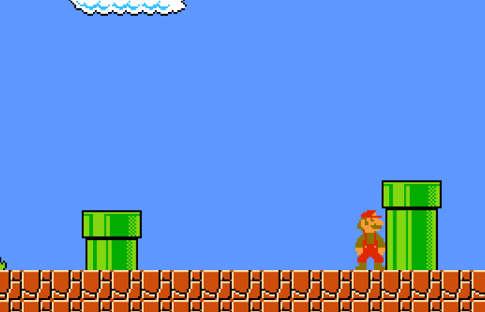
\includegraphics[scale=0.55]{pictures/Mario1.PNG}
	\caption{Mario has to go left in order jump over the obstacle}
	\label{fig:marioLeft}
\end{figure}
\begin{figure}[!h]
	\centering
	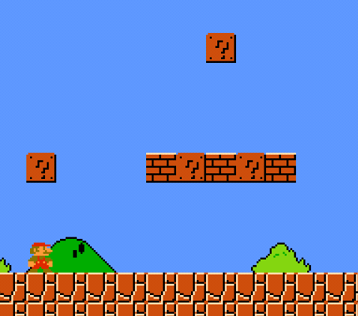
\includegraphics[scale=0.55]{pictures/Mario2.PNG}
	\caption{Mario with loot boxes over him}
	\label{fig:marioSmashHead}
\end{figure}
\begin{figure}[!h]
	\centering
	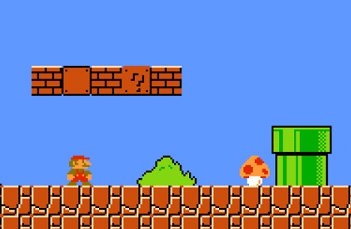
\includegraphics[scale=0.55]{pictures/Mario3.PNG}
	\caption{Mario with a mushroom}
	\label{fig:marioEat}
\end{figure}
\begin{figure}[!h]
	\centering
	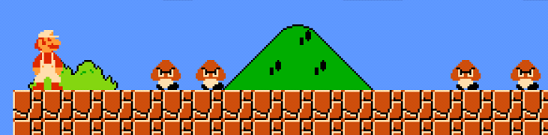
\includegraphics[scale=0.55]{pictures/Mario4.PNG}
	\caption{Mario with enemies}
	\label{fig:marioFight}
\end{figure}

\subsection{Preparations (by Haller and Heithoff)}
The Code of the PacMan emulator \cite{pacmanLink} and SuperMario emulator \cite{marioLink} we used was available in Html5 and JavaScript. C\&C-Components in EmbeddedMontiArc can be translated to C++ code and then to a web assembly (using Emscripten \cite{emscirpten}) which uses JavaScript (see \cite{bertram2017component}). This JavaScript file can be given inputs according to the component and calculates the outputs on execution. To combine these two files, there is an additional interface needed to extract the information for the inputs out of the emulator and then give the calculated outputs into the emulator.
For the purpose of implementing the controllers the subjects were assigned to use the EmbeddedMontiArcStudio.
EmbeddedMontiArcStudioV1.6.2 did neither support a simulator of PacMan nor of a simulator SuperMario. So an additional step to answer RQ2 \textit{Is it possible to integrate other simulators in a recent amount of work} it for the groups to integrate the simulators into the EmbeddedMontiArcStudio.

In order to be able to do so, group A is instructed by an expert (Jean-Marc) which files need modification and what to add. After that group A instructed group B the same way.

